\documentclass{llncs}
\usepackage{makeidx}
\usepackage[utf8]{inputenc}
%\usepackage{graphics}
%\usepackage[pdftex]{graphicx}
\usepackage{listings}
\usepackage{graphicx}  

\begin{document}

\title{Waypoint navigation for an airplane UAV using MAVlink in JdeRobot framework}
\author{José Antonio Fernández\inst{1} \and Jose María Cañas Plaza\inst{2}}
\institute{Universidad Rey Juan Carlos}
\titlerunning{Article Abv}
\maketitle

\begin{abstract}
In order to make accesible to \texttt{JdeRobot} the command sets of \texttt{MAVLink} a driver is needed. The \texttt{APM Server driver} ``translates'' the \texttt{JdeRobot} interfaces objects in \texttt{MAVLink's} commands an viceversa, giving access to sensors and actuators of the robot. With the typical \texttt{JdeRobot} architecture applications can run in different machines (not necessarily aboard) and can be writen in different programming languages. 
In our case this driver run in a \texttt{Raspberry Pi3} with \texttt{raspbian OS} aboard the plane
\end{abstract}

\section{Introduction}

%MAVlink protocol

\section{UAV support in JdeRobot}

\section{MAVlink protocol}

\section{APM driver in JdeRobot}

\subsection{Design}
\label{sec:design}

The driver has to fullfil the following features:

\begin{itemize}
\item Have to be able to connect to a physical devices like APM 2.8 but as well as to a simutator.
\item Have to access to sensors measures of the aereal robot and interpreting the data and serve its as ICE interfaces objects.
\item Have to be able to recieve incoming commands as ICE interfaces objects and send its to the devices as \texttt{MAVLink's} commands.
\end{itemize}

\begin{figure}[h]
  \centering
  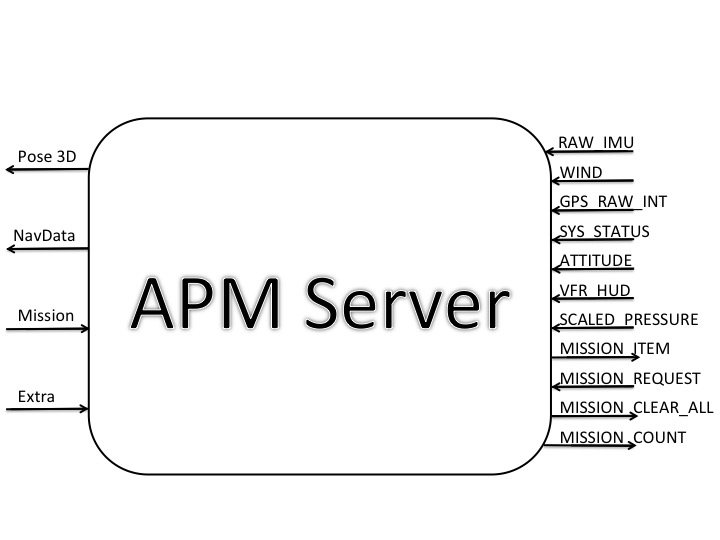
\includegraphics[scale=0.5]{img/diseno.jpg}
  \caption{Diseño de entradas y salidas de \texttt{APM Server}}
  \label{fig:diseno_apms_caja_negra}
\end{figure}

In order to adress it, a Python in \texttt{JdeRobot} component has been developed who implements all of above features called \texttt{APM Server}. 
\texttt{APM Server} is organized in three logical layers.
\begin{itemize}
\item Comunication's layer with APM's devices. ensures the establishment and maintenance the comunication with the APM device through \texttt{MAVLink's} commands.
\item Bussiness Layer. In this layer the driver convert form \texttt{MAVLink's} commands to ICE interfaces objects and viceversa.
\item \texttt{JdeRobot comunication's layer} This layer create all the ICE servers needed and handle incoming and outgoing ICE interfaces objects.
\end{itemize}
\begin{figure}[h]
\centering{
   \label{f:diseno_apms_caja_trans}
    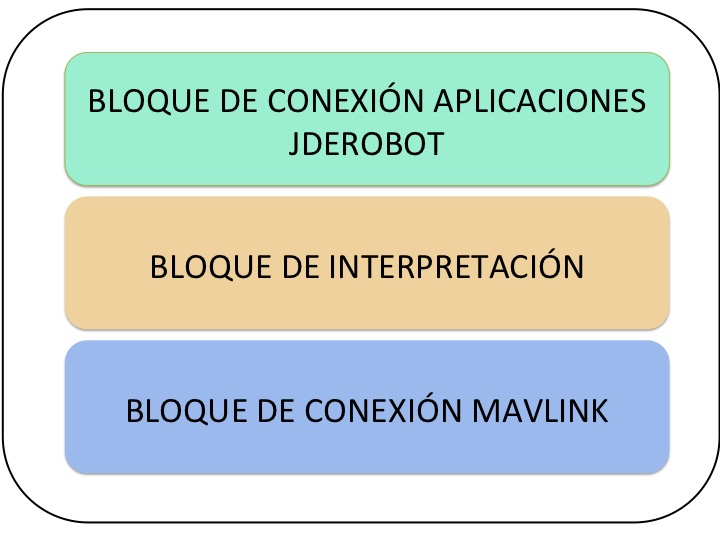
\includegraphics[width=0.7\textwidth]{img/diseno1.jpg}}
    \caption{Bloques del driver \texttt{APM Server}}
  
\end{figure}

\subsection{Comunication with APM devices layer}
\label{sec:apm_comunication}
% Always give a unique label
% and use \ref{<label>} for cross-references
% and \cite{<label>} for bibliographic references
% use \sectionmark{}
% to alter or adjust the section heading in the running head

In this layer the driver send the \texttt{MAVLink's} commands and recieve the \texttt{MAVLink's} messages which conform the comunication with the APM device.
The driver have to understand the APM device's messages received in \texttt{MAVLink} protocol as well as build this commands and send it to the APM.

\subsubsection{MAVLink's message}

The driver handle 11 commands of the full set of \texttt{MAVLink's} commands (see Figure 3.1) to allow the \texttt{JdeRobot} integration. Below it's described one of them in order to know this protocol.

\begin{verbatim}
<message id="33" name="GLOBAL_POSITION_INT">
	<description>The filtered global position 
	(e.g. fused GPS and accelerometers). The 
	position is in GPS-frame (right-handed, Z-up).
	It is designed as scaled integer message 
	since the resolution of float is not 
	sufficient.	</description>
<field type="uint32_t" name="time_boot_ms" units="ms">
	Timestamp (milliseconds since system boot)</field>
<field type="int32_t" name="lat" units="degE7">Latitude, 
	expressed as degrees * 1E7</field>
<field type="int32_t" name="lon" units="degE7">Longitude, 
	expressed as degrees * 1E7</field>
<field type="int32_t" name="alt" units="mm">Altitude in 
	meters, expressed as * 1000 (millimeters)</field>
<field type="int32_t" name="relative_alt" units="mm">
	Altitude above ground in meters, expressed as 
	* 1000 (millimeters)</field>
<field type="int16_t" name="vx" units="cm/s">Ground X 
	Speed (Latitude, positive north), expressed as 
	m/s * 100</field>
<field type="int16_t" name="vy" units="cm/s">Ground Y 
	Speed (Longitude, positive east), expressed as 
	m/s * 100</field>
<field type="int16_t" name="vz" units="cm/s">Ground Z 
	Speed (Altitude, positive down), expressed 
	as m/s * 100</field>
<field type="uint16_t" name="hdg" units="cdeg">Vehicle 
	heading (yaw angle) in degrees * 100, 0.0..359.99 
	degrees. If unknown, set to: UINT16_MAX</field>
</message>
\end{verbatim}

One example of this incoming message is:
\begin{verbatim}
GLOBAL_POSITION_INT {time_boot_ms : 480614, lat : -
353632612, lon : 1491652301, alt : 584110, 
relative_alt : -179, vx : 0, vy : 0, vz : 0, hdg : 
35608}
\end{verbatim}

\subsubsection{Setup and APM connection}

As has been showed the APM comunication is under \texttt{MAVLink} so the setup and conection have its own commands in this protocol.
To help us to build and understand these messages the driver uses \texttt{pymavlink}.

The connection is established in the server object creation, in the \_\_init\_\_() method of the class. The connection command needs two parameters: the device and the connection speed in bauds.
{\scriptsize
\begin{lstlisting}
classServer:
	def__init__(self,port,baudrate):
		self.master=mavutil.mavlink_connection(port,
					baudrate,autoreconnect=True)
		self.master.wait_heartbeat()
		...
__init__()
#test=Server("/dev/ttyUSB0",57600)#ConnectiontotherealAPMdevice
test=Server("udp:192.168.1.133:14558",57600)#ConnectiontoSITL
\end{lstlisting}}

The last two sentences shows an example of a real device connection and SITL's connection respectively.

Once the connection is made, the AMP \texttt{MAVLink's} messages start to be stored in a buffer, and we can setup it. The incoming messages rate and the set of these command we need are configurable parameters. Set up it is easy as is showed in the following lines.

{\scriptsize
\begin{lstlisting}
RATE=50
self.master.mav.request_data_stream_send(self.master.target_system,
						self.master.target_component,
						mavutil.mavlink.MAV_DATA_STREAM_ALL,
						RATE,1)
\end{lstlisting}}

The available set connections are:

\begin{verbatim}
MAV_DATA_STREAM_ALL	Enable all data streams
MAV_DATA_STREAM_RAW_SENSORS	Enable IMU_RAW, 
	        GPS_RAW, GPS_STATUS packets.
MAV_DATA_STREAM_EXTENDED_STATUS	Enable GPS_STATUS, 
	        CONTROL_STATUS, AUX_STATUS
MAV_DATA_STREAM_RC_CHANNELS	Enable RC_CHANNELS_SCALED,
	        RC_CHANNELS_RAW, SERVO_OUTPUT_RAW
MAV_DATA_STREAM_RAW_CONTROLLER	Enable 
	        ATTITUDE_CONTROLLER_OUTPUT, 
	        POSITION_CONTROLLER_OUTPUT, 
	        NAV_CONTROLLER_OUTPUT.
MAV_DATA_STREAM_POSITION	Enable LOCAL_POSITION, 
	        GLOBAL_POSITION/GLOBAL_POSITION_INT messages.
MAV_DATA_STREAM_EXTRA1	Dependent on the autopilot
MAV_DATA_STREAM_EXTRA2	Dependent on the autopilot
MAV_DATA_STREAM_EXTRA3	Dependent on the autopilot

\end{verbatim}

And the RATE value depends of the choosed device.


\subsubsection{APM data reading}
\label{subsec:apm_data_reading}

In order to retrieve the APM sensors measures, a thread is ejecuting a message handler all the time.
In this handler the method search for seven types of messages (like GLOBAL\_POSITION\_INT) which contains the needed data to fill the two ICE interfaces that the server serves: \texttt{Pose3D} y \texttt{NavData}.


\subsubsection{Sending missions to APM}
\label{sec:mission_apm}

This is the most important part of the driver. The driver recieve two ICE interfaces, one developed in this project called \texttt{mission} with the waypoints to follow and the \texttt{Extra} interface with the take off and land maneuvers.
Once a mission is received through these interfaces objects, \texttt{APM Server} build the \texttt{MAVLink's} commands needed to sent it to the APM. To perform it, a new thread with a listener was developed in order to know if there is a incominf mission.
Once this listener detects an incoming mission, call to \texttt{setMission(self, mission)} who build the \texttt{MAVLink's} commands and sent it as the Figure 3.3 diagram shows.
The \texttt{setMission(self, mission)} method read througth the list of waypoints and if \texttt{takeOffDecision} and \texttt{landDecision} of \texttt{Extra} object are seted to True add the \texttt{MAVLink's} commands of take off and land at first and last of the list of commans whitch is sended to the APM.
 

\begin{figure}[h]
  \centering
  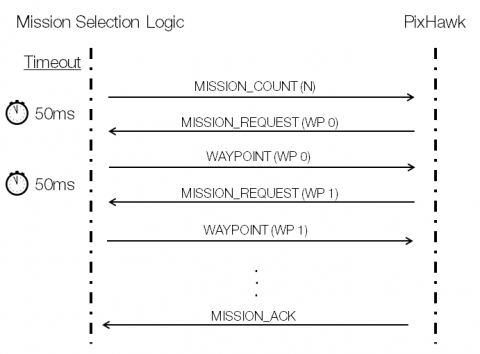
\includegraphics[scale=0.70]{img/waypoint-protocol-sendlist.png}
  \caption{\texttt{MAVLink's} missions sending protocol}
  \label{fig:misiones_mavlink}
\end{figure}

\subsection{Connection to applications layer}
\label{sec:apm_jderobot_comunication}

In this layer all the ICE interfaces objects are handled. The driver uses four interfaces. Two of there are served (outgoing), \texttt{Pose3D} and \texttt{NavData} and the rest are received: \texttt{mission} and \texttt{extra}.
Each interfaces has its own thread with its own ICE server (note that ICE servers communication are bidirectional, so in this case ``server'' word don't refer to the side of the data).
In the following lines an ICE server implementation are showed.
{\scriptsize
\begin{lstlisting}

def openPose3DChannel(self, pose3D):
   status = 0
   ic = None
   Pose2Tx = pose3D
   try:
       ic = ICE.initialize(sys.argv)
       adapter = ic.createObjectAdapterWithEndpoints("Pose3DAdapter", 
       				"default -p 9998")
       object = Pose2Tx
       adapter.add(object, ic.stringToIdentity("ardrone_pose3d")) 
       adapter.activate()
       ic.waitForShutdown()
   except:
       traceback.print_exc()
       status = 1
   if ic:
       try:
           ic.destroy()
       except:
           traceback.print_exc()
           status = 1
   sys.exit(status)
\end{lstlisting}}

\subsection{Interpretation layer}
\label{interpretation_layer}

This layer makes all the needed data's tranformation. So once the \texttt{MAVLink's} message is located, this layer makes it fit in the corresponding ICE interfaces and the same in opposite side communication. 
The \texttt{setMission(self, mission)} and the \texttt{refreshAPMPose3D()} and
\texttt{refreshAPMnavdata()} are the most important methods involved in this layer.

\section{UAV Commander application}

\section{Conclusions}

\end{document}
